%%%%%% CMB-S4 Simulations and Data Analysis Chapter, Component Separation Section  %%%%%%%%%%%%%%%%

\section{Component Separation}

\textbf{ Authors: Mark Ashdown, Jonathan Aumont, Carlo Baccicalupi, Josquin Errard, Maude Le Jeune}

Key challenges:
\begin{itemize}
\item validation - are we using the right algorithms for the (as yet unknown) real foregrounds
\item verification - are these algorithms right given our (as yet flawed) simulations
\end{itemize}

\begin{figure*}[htbp]
\centering
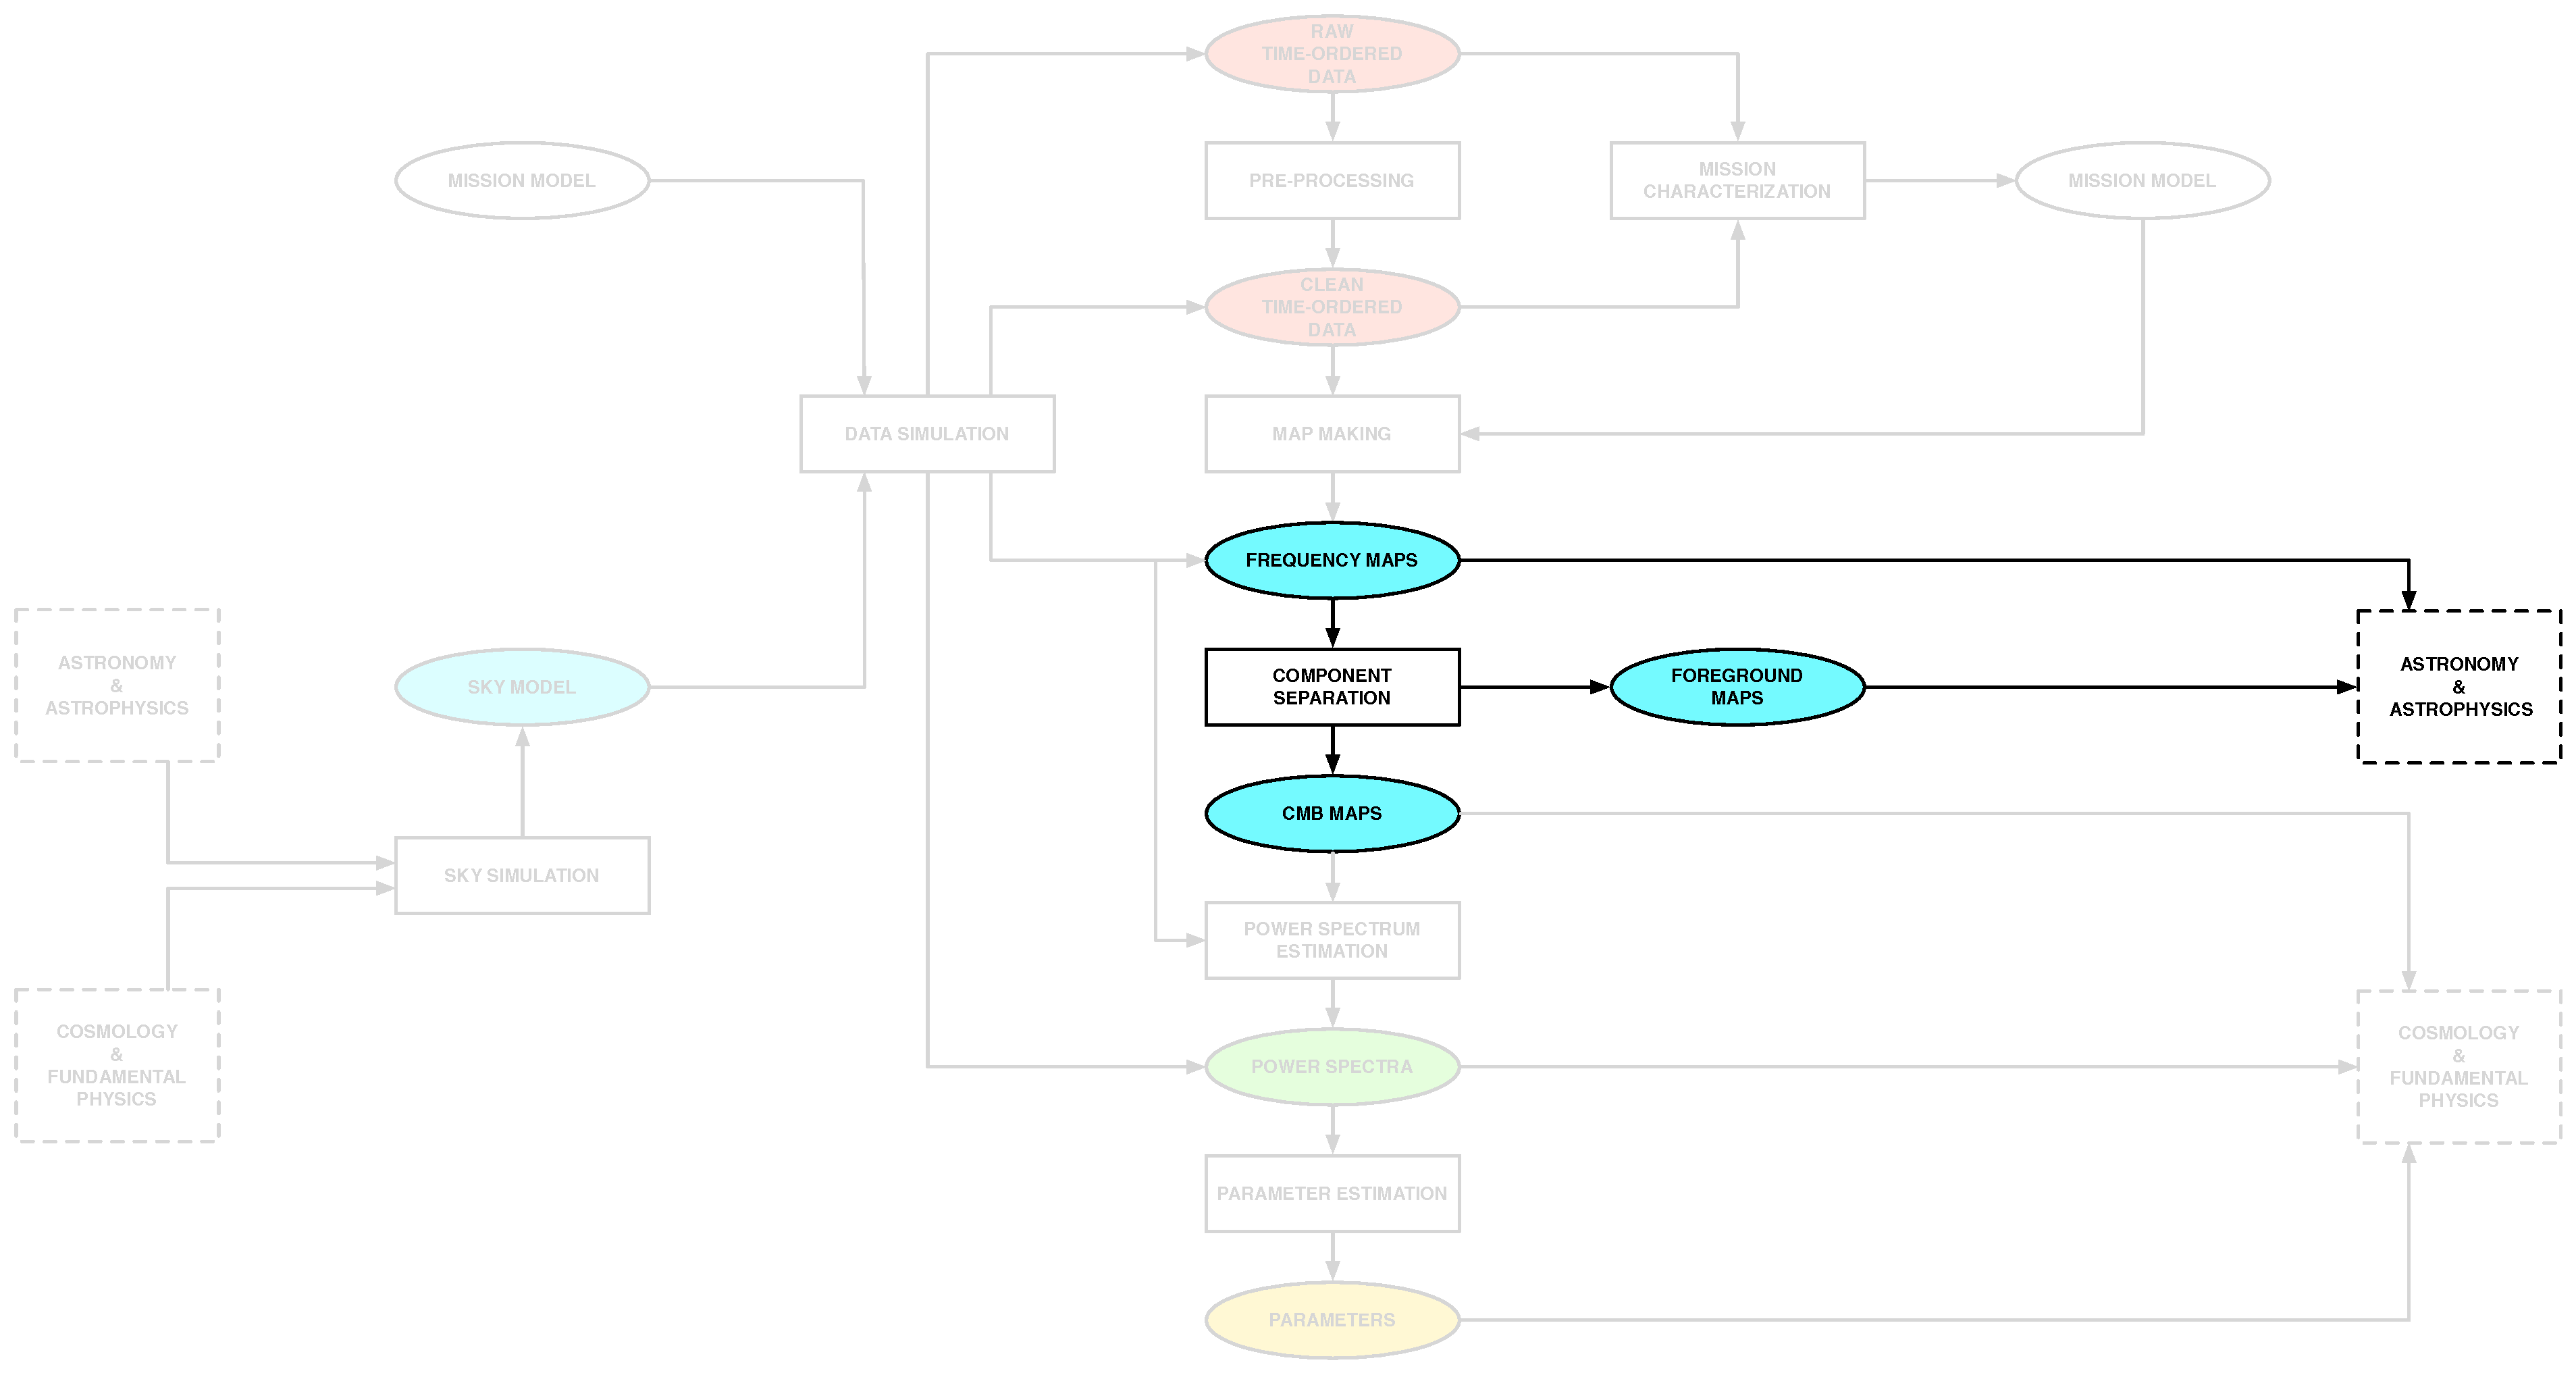
\includegraphics[width=1\textwidth]{Analysis/cs}
\caption{The component separation components of the CMB simulation and data analysis pipeline}
\label{default}
\end{figure*}


\subsection{Introduction}


\subsubsection{Motivations}

S4 science goals are r and neutrino mass
\begin{itemize}
	\item component separation is obviously a necessary step to go beyond current constraints on e.g. prim B-modes, cf. e.g. Fig.  of Errard et al (2015)?
	\item for neutrino mass, I suppose $C_\ell^{dd}$ has the best lever-arm, and we should evaluate the impact of foregrounds on the 4-point function (E-B estimators I suppose). NB: Planck lensing 2015 is based on SMICA map.
\end{itemize}

%%%%%%%%%%%%%%%%%%%%%%
\subsubsection{Definition of component separation}
\begin{itemize}
	\item includes any data processing that characterizes and exploits correlations between multi-frequencies observations,
	\item puts external constraints and physical modeling
	\item and it aims at distinguishing between different physical sources of emission.
	NB For a given method, one would think that there should be a validation step (do the tools work on reasonable sky models?) and a verification step (are the sky models consistent with reality?). The second step is obviously the most difficult to answer.
\end{itemize}

$\rightarrow$ feedback from Planck component separation as well as the early CMB cleaning achieved in the BKP measurements + Stivoli et al (2010) + Fantaye et al (2011+2012) + Errard et al (2011+2012+2015).

%%%%%%%%%%%%%%%%%%%%%%
\subsection{Description of methods}
\begin{itemize}
	\item Parametric
	\item Blind
	\item Discussion regarding the domain of application (harmonic, pixel, wavelet,etc.)
\end{itemize}

$\rightarrow$ Parametric fitting vs. ILC, spatial domain versus
non-spatial, that makes a basis of 4 algorithms. Although it was never
quantified, the independence of those and very different hypotheses represent
an opportunity for cross-checking and robustness.

%%%%%%%%%%%%%%%%%%%%%%
\subsection{Questions to be addressed during follow-up studies}
\begin{itemize}
	\item pros/cons for E/B vs Q/U
	\item pros/cons for multi-sites
	\item pros/cons for having various resolutions
	\item atmosphere residuals and dust in maps could scale similarly with frequency...
	\item we could outline a roadmap, i.e. the application and learning phase to SIV made by the various sub-orbitals which are going on-line now or soon with the usual 95, 150, 220. That would need to be investigated very accurately as it would represent a most important step for component separation
towards SIV.
\end{itemize}





%\bibliography{cmbs4}

%%
%% Populate the .bib file with entries from SPIRES Bibtex (preferred)
%% or ADS Bibtex (if no SPIRES entry).
%%  SPIRES will also supply the CITATION line information; please include it.
%%


